% Chapter 4

\chapter{Methodology} % Write in your own chapter title
\label{Chapter4}
\lhead{Chapter 4. \emph{Methodology}} % Write in your own chapter title to set the page header
In this chapter we introduce and describe the real life game dataset that we got from GameAnalytics (GA), selection of user events and building player behavior features to construct a game metric data as input to our clustering algorithm. In GA the user telemetry data arrives in mini batches from the games, a batch each day. In this thesis the idea is then to process each batch and incrementally cluster the data, where the output from one batch is the input to the next.

We implemented a incremental MapReduce (MR) k-means clustering algorithm and apply it on multiple batches of the game metric data to find average player behaviors described by a the constructed player behavioral feature vector. The algorithm is highly scalable and can easily be executed on numerous virtual computers using the Amazon Elastic MapReduce (Amazon EMR) web service. 

We test the MR k-means algorithm on multiple batches of the real game data. Where each batch of game data is processed in one iteration and the output is used as the input to the next batch. Using one iteration we allow for efficient computation and given the changing nature of the data over time in each batch we don't risk falling into local optimum. This method is compared against multiple iterations on the real game data and on a larger generated example, where 3 normal distributions shift between data batches.

Different MR k-means implementation were tried in the process of the thesis and different efficient computational methods were compared on a larger generated dataset, including scalability (scale-up and scale-out) tests running on different cluster setups in the Amazon EMR.

\section{Dataset}
The dataset is from a Free-to-Play (F2P) online game that is available on Google Plus and Facebook. This real life game dataset is from one of the many games that GameAnalytics is analyzing for their customers. Because of confidentiality issues we are not allowed to mention its name but lets call it \textit{Free Battle Online} (FBO). Same is about the real names of events or features in the dataset is fictional, this unfortunately means that we also have very limited knowledge about the data, e.g. what individual events mean and the timespan. The goal of FBO is to fight battles against both non-playing-characters (NPCs) and other players. You can click on various places to travel to finish battle missions or just visit other players and initiate battles to steal their resources.

The dataset is a user telemetry data, e.g. user behavioral events, where each line represents an action performed by the user or is a direct influence from a user behavior. There are over $5.000.000$ rows in this data set, with approx. $550$ unique events generated by approx. $94.000$ players. Average events per player is $\mu = 54$ with standard deviation $\sigma = 145$, indicating that the data is spread out over a wide range of values. The measure of the spread is in Table~\ref{tab:FiveSummaryEvents} showing the five number summary; The first quartile $Q_1$ cuts off the lowest $25\%$ of the data, the second quartile gives the center of the distributions known as the $Median$, the third quartile $Q_3$ cuts of the highest $25\%$. The median is lower than the mean of the data describing a positively skewed distribution, see Figure~\ref{fig:boxplot_events} for a visualization of the distribution.

\begin{table}[h]
\centering
\begin{tabular}{| l | l | l | l | l | l |}
    \hline
    & \textit{Min} & $Q_1$ & \textit{Median} & $Q_3$ & \textit{Max} \\ \hline
    Events & 1 & 4 & 23 & 61 & 10865 \\ \hline
\end{tabular}
\caption{This table shows the five number summary about the number of events generated by each unique player in the dataset.}
\label{tab:FiveSummaryEvents}
\end{table}


\begin{figure}[here]
\centerline{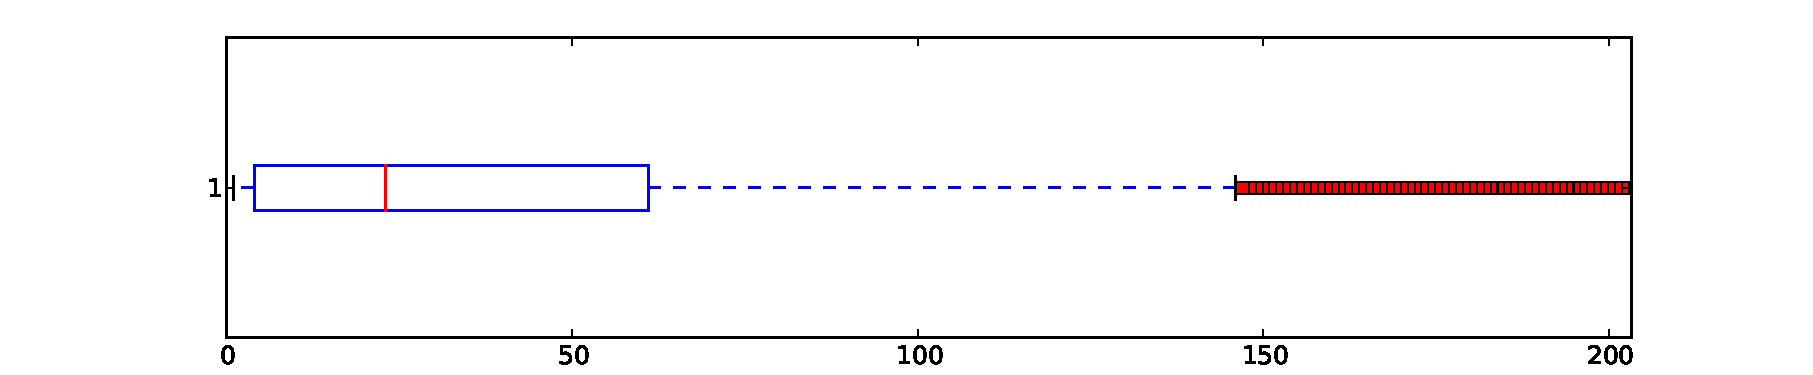
\includegraphics[width=0.9\textwidth]{Figures/boxplot_events.pdf}}
\caption{A boxplot visualizing the Events distribution incorporating the five number summary.}
\label{fig:boxplot_events}
\end{figure}

The two lines outside the box in Figure~\ref{fig:boxplot_events} are called whiskers and represent the extreme low and high values that are less than $1.5 \times IQR$ beyond the quartiles. The first and third quartiles represent the ends of the box and the median is the red line. The red \textit{squares} are individual points called \textit{outliers}. Only about $6\%$ or $\approx 5500$ players of the entire population generated more than 150 events, $0.3\%$ or $\approx300$ players have more than 1000 events and less than ten people have a range of $5.000-10.000$ generated events! A histogram showing the frequency of events generated by players is shown in Figure~\ref{fig:histogram_events_iqr}, zooming in on the spread that gives the range covered by the middle half of the data.

\begin{figure}[here]
\centerline{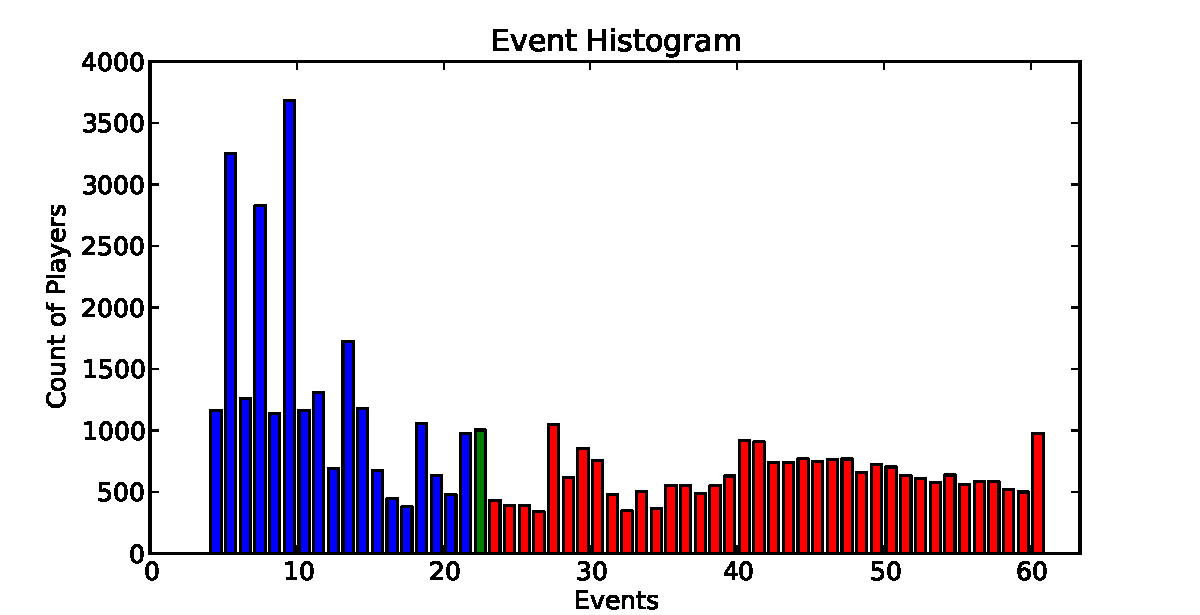
\includegraphics[width=0.9\textwidth]{Figures/histogram_events_iqr.pdf}}
\caption{A histogram for number of events using singleton buckets in the interquartile range (IQR) defined as $Q3 - Q1$, range covered by the middle half of the data.}
\label{fig:histogram_events_iqr}
\end{figure}


\subsection{Game Metric Construction}
\label{gamemetric}
For this thesis we tried to keep the number of game features in minimal and decided to build our feature vector with three features. Given the limited knowledge and information that we have about individual events we decided to select events that have high frequency compared to other events and hopefully could describe different behaviors between groups of players in those features. A $3-dimensional$ feature vector was constructed for each unique player, containing a frequency of three events generated by the player. The aggregated events are:
\begin{itemize}
\item Login: Number of logins/access into different areas in the game($\mu = 2.4, \sigma = 4.8$)
\item Battle: Number of battles this player have started ($\mu = 3.7, \sigma = 9.6$)
\item Premium Spending: Number of times this player spends a in-game money on virtual items or resources ($\mu = 1.1, \sigma = 2.7$) 
\end{itemize}

We tried to chose features that could describe player engagement to the game. How active the player is exploring various areas, fighting battles and spending in-game money to advance in the game quicker. The five number summary of the skewed distribution is in Table~\ref{tab:FiveSummaryLoginsBattlesPremium}. Boxplots visualizing the distributions for these events are shown in relevant figures below, Logins in Figure~\ref{fig:boxplot_logins}, Battles in Figure~\ref{fig:boxplot_battles} and Premium spent events in Figure~\ref{fig:boxplot_premium}.


\begin{table}[h]
\centering
\begin{tabular}{| l | l | l | l | l | l |}
    \hline
    & \textit{Min} & $Q_1$ & \textit{Median} & $Q_3$ & \textit{Max} \\ \hline
    Logins & 0 & 1 & 1 & 2 & 220 \\ \hline
    Battles & 0 & 0 & 1 & 4 & 439 \\ \hline
    Premium spent & 0 & 0 & 0 & 1 & 100 \\ \hline
\end{tabular}
\caption{This table shows the five number summary for the Logins, Battles and Premium spent events generated by each unique player in the dataset.}
\label{tab:FiveSummaryLoginsBattlesPremium}
\end{table}

The features values are spread out over large range of values, in the preprocessing Section~\ref{preprocessing} we explain how we detect and remove the outliers or anomalies from our data before we apply our MR k-means algorithm using a \textit{z-score} method.

\begin{center}
\begin{figure}[h]
\centerline{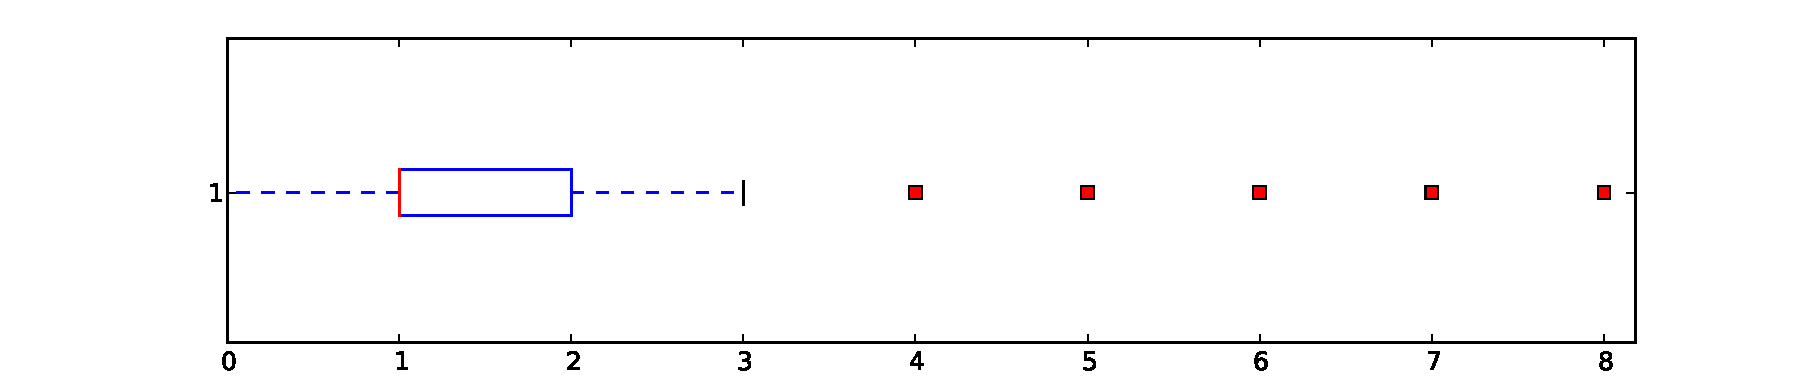
\includegraphics[width=0.9\textwidth]{Figures/boxplot_logins.pdf}}
\caption{A boxplot visualizing the Login events distribution incorporating the five number summary.}
\label{fig:boxplot_logins}
\end{figure}

\begin{figure}[h]
\centerline{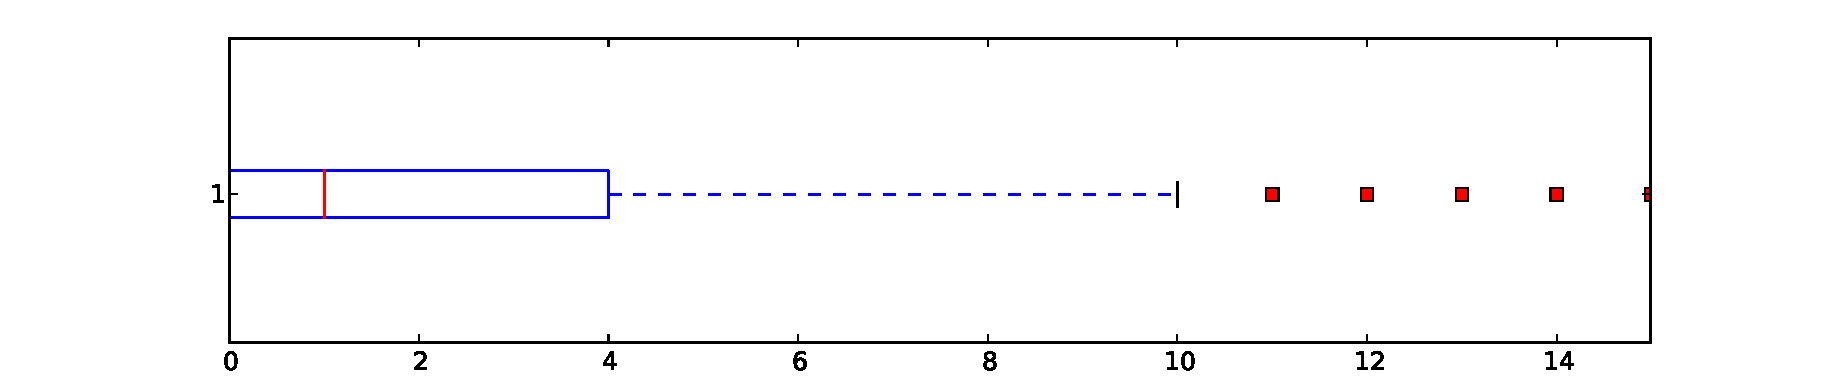
\includegraphics[width=0.9\textwidth]{Figures/boxplot_battles.pdf}}
\caption{A boxplot visualizing the Battle events distribution incorporating the five number summary.}
\label{fig:boxplot_battles}
\end{figure}

\begin{figure}[here]
\centerline{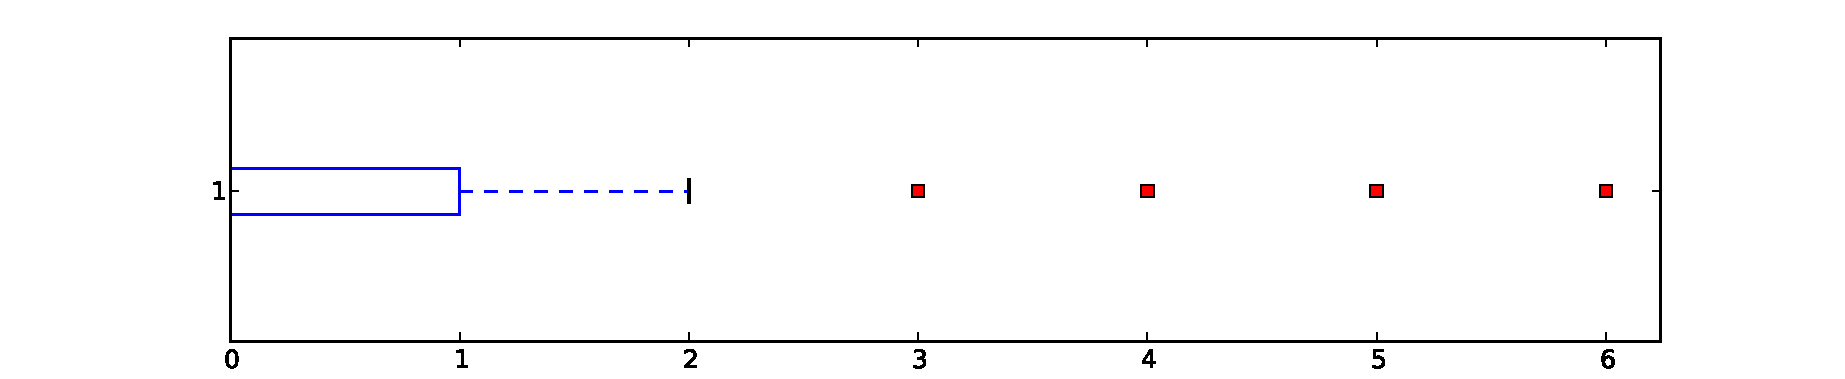
\includegraphics[width=0.9\textwidth]{Figures/boxplot_premiumspent.pdf}}
\caption{A boxplot visualizing the Premium spent events distribution incorporating the five number summary.}
\label{fig:boxplot_premium}
\end{figure}
\end{center}


\subsection{Preprocessing}
\label{preprocessing}
User telemetry from games can be very noisy in that sense it can contain lots of irrelevant events and logging information and even developers from the game studio can generate events. For this dataset this we performed several preprocessing steps:
\begin{itemize}
\item Sort the events after event timestamp.
\item Split the dataset into $10$ approx. equally sized data set pieces.
\item Filter out irrelevant events and logging information. E.g. Events not origin from Facebook or Google Plus, non related events and in game studio debugging generated events.
\item For each data set piece:
 \begin{itemize}
 \item Counting the events mentioned above per user to build our feature vector.
 \item Remove outliers or anomalies from the data.
 \item Standardize the data to standard scores also called \textit{z-score}. Transforming the data
to standard normal distribution, with $\mu = 0$ and $\sigma = 1$. 
 \end{itemize}
\end{itemize}

To apply our incremental MR k-means algorithm we need to have multiple batches of data to process incrementally. We use the real game dataset that we got from GA and split it up into $10$ equally sized data batches sorted after the event arrival timestamp. By doing so we try to simulate that we are processing multiple batches of data in the same order as the events were generated over mulitple time-periods or days, like at GA. Next we filter out irrelevant information, e.g. information that don't contribute as a event logging or are obviously from the game designers themselves.

When processing each data batch we aggregate or count the events that we selected before to build our feature vector for each unique player in the data set. Next we find the outliers by transforming the data to standard scores using the \textit{zero mean normalization} (ZMN), also called \textit{z-score}, with standard normal distribution having zero mean and unit variance $\mu = 0$ and $\sigma = 1$. A feature vector that has a feature value z-score that is more than $3$ standard deviations away from the mean is considered an outlier in the data and is removed from the original data batch. Having a data batch without outliers we now can transform the data again using ZMN, without having the outliers to effect our transformation. The ZMN is defined as follows


\begin{center}
$z = \dfrac{x  - \mu}{\sigma}$ 
\end{center}


Using ZMN is widely used in machine learning algorithms and is needed when calculating the distance between two points (feature vectors) such that each feature contributes approximately equally to the final distance.

Removing the outliers from the whole dataset, using the ZMN method described above, the total number of unique players become approx $90.800$ instead of approx. $94.000$, removing $\approx 4\%$ of the population. The five number summary for the whole dataset can be found in Table~\ref{tab:FiveSummaryLoginsBattlesPremiumWoOutliers}, notice the range of values compared to the Table~\ref{tab:FiveSummaryLoginsBattlesPremium} in Section~\ref{gamemetric}. The multiple data batches that we feed into our clustering algorithm had $\approx 5\%$ player feature vectors removed on average, see Table~\ref{tab:DatabatchesWoOutliers} below.

\begin{table}[h]
\centering
\begin{tabular}{| l | l | l | l | l | l |}
    \hline
    & \textit{Min} & $Q_1$ & \textit{Median} & $Q_3$ & \textit{Max} \\ \hline
    Logins & 2 & 1 & 1 & 2 & 16 \\ \hline
    Battles & 0 & 0 & 1 & 4 & 32 \\ \hline
    Premium spent & 0 & 0 & 0 & 0 & 9 \\ \hline
\end{tabular}
\caption{This table shows the five number summary for the Logins, Battles and Premium spent events generated by each player from the whole dataset with outliers removed.}
\label{tab:FiveSummaryLoginsBattlesPremiumWoOutliers}
\end{table}


\begin{table}[h]
\centering
\scalebox{0.8}{%
\begin{tabular}{| l | l | l | l | l | l | l | l | l | l | l |}
    \hline
    & Data 1 & Data 2 & Data 3 & Data 4 & Data 5 & Data 6 & Data 7 & Data 8 & Data 9 & Data 10 \\ \hline
    Players & 14054 & 13365 & 13403 & 13503 & 13441 & 13276 & 12839 & 13413 & 13473 & 13412 \\ \hline
    Outliers  & 658 & 741 & 661 & 673 & 748 & 698 & 685 & 724 & 669 & 680 \\ \hline
    $\%$ removed & $4,68\%$ & $5,44\%$ & $4,93\%$ & $4,98\%$ & $5,56\%$ & $5,25\%$ & $5,33\%$ & $5,39\%$ & $4,96\%$ & $5,07\%$ \\ \hline
\end{tabular}}
\caption{This table shows the player population, number of outliers found and the percentage of the population removed, for each data batch.}
\label{tab:DatabatchesWoOutliers}
\end{table}



\section{K-means algorithm in MapReduce}
A k-means algorithm was implemented in MapReduce (MR) that is able to incrementally process large-scale datasets in parallel when running on e.g. Amazon EMR. We implemented two versions of MR k-means that use different MR execution flows. We first started to implement a naive and a common implementation version of MR k-means that assigns each point (feature vector) to a nearest cluster in the \textit{Map} phase and updates the centroids for the clusters in the \textit{Reduce} phase. The programmer only needs to fill in two functions, the Map and Reduce. The other version has a \textit{Combiner} phase implemented that performs a reduce work on the same computer node as the Mapper, by calculating intermediate sums of all the points for each cluster from a Map function. This minimizes the data needed to be transferred and shuffled by the MR framework to the Reducer, sending only an intermediate sum with each centroid from each mapper instead of list of all data points belonging to each cluster \citep{Dean:2004}. The second implementation using a Combiner is used in the experiments (with some efficiency adjustments) where we cluster the real game data, since it is a more efficient and scalable when processing larger amount of data as explained in Section~\ref{sec:MRLargeData} and Section~\ref{sec:MapCombineReduceVersion} and as result show from experiments in Chapter~\ref{Chapter5}.

In the next two subsections we will describe the two implementations and their pseudo codes. Then we will explain the \textit{Incremental MRK-means Program} that controls the incremental data batch processing by executing $n$ iterations of the MRK-means job. The most computational expensive part in k-means is to find the nearest centroid for a given feature vector by calculating the distance between the two. We implemented three different distance calculation versions to find the most efficient one when running on a cluster setup using Amazon EMR. In the last subsection  we give a quick overview of the development environment and tools that were used in this thesis.

\subsection{K-means version 1 - Map and Reduce}
Implementing the Map and a Reduce function version is the most common implementation of k-means in MR. Where The Map function calculates the nearest centroids to each data point and emits that pair to the Reduce function that sums up all data point values for each centroid and outputs updated centroids. Our Map function is called for each player feature vector found in the data batch and we iterate through all centroids that we have in memory to calculate the distance to the nearest one. The nearest centroid and its data feature vector is emitted from all the Map tasks running in parallel to the MR framework that shuffles and sorts all feature vectors together belonging to the same centroid. The pseudo-code for the Map function can be found in Algorithm~\ref{alg:mapkmeansv1} and for Reduce in Algorithm~\ref{alg:reducekmeansv1}.

\algsetup{indent=2em}
\begin{center}
\newcommand{\map}{\ensuremath{\mbox{\sc Kmeans version 1: Map}}}
\begin{algorithm}[h!]
\caption{$\map(key,value)$}\label{alg:mapkmeansv1}
\begin{algorithmic}[1]
\REQUIRE $key = document\_name$, $value = feature\_vector$
\ENSURE $key = centroid\_id$, $value = feature\_vector$.
\STATE $current\_centroids \leftarrow C = \{c_1...c_k\}$ \COMMENT{loaded into memory}
\STATE $feature\_vector \leftarrow = value$
\medskip
\STATE  $mindist \leftarrow +\infty$
\STATE $minCentroid \leftarrow None$
\FORALL{$centroid \in  current\_centroids$} 
	\STATE $distance \leftarrow getDistance(feature\_vector, centroid) $
	\IF{$distance < mindist$ \OR $minCentroid = None$} 
		\STATE $mindist \leftarrow distance$
		\STATE $minCentroid \leftarrow centroid$ \COMMENT{nearest centroid}
	\ENDIF
\ENDFOR
\medskip
\STATE{$EmitIntermediate(minCentroid, feature\_vector)$}
\end{algorithmic}
\end{algorithm}
\end{center}

\begin{center}
\newcommand{\map}{\ensuremath{\mbox{\sc Kmeans version 1: Reduce}}}
\begin{algorithm}[h!]
\caption{$\map(key,value)$}\label{alg:reducekmeansv1}
\begin{algorithmic}[1]
\REQUIRE $key = centroid\_id$, $values = feature\_vector\_list$
\ENSURE $key = centroid\_id$, $value = average\_feature\_vector$.
\STATE $feature\_vector\_list \leftarrow values$
\medskip
\STATE $sum\_feature\_vector \leftarrow [0, 0, 0]$
\FORALL{$feature\_vector \in  feature\_vector\_list$} 
	\STATE $sum\_feature\_vector \leftarrow sum\_feature\_vector + feature\_vector$
\ENDFOR
\medskip
\STATE $count\_feature\_vectors \leftarrow getCount(feature\_vector\_list)$
\STATE $average\_feature\_vector \leftarrow sum\_feature\_vector \div count\_feature\_vectors$
\medskip
\STATE{$EmitIntermediate(key, average\_feature\_vector)$}
\end{algorithmic}
\end{algorithm}
\end{center}

The Reduce function then gets one input per centroid and all its feature vectors. Iterating through all the feature vectors, summing up their values and divide with their count to get a new updated centroid and outputs that centroid or the mean that represents the average feature vector for the cluster population.


\subsection{K-means version 2 - Map, Combiner and Reduce}
\label{sec:MapCombineReduceVersion}
By adding the Combiner phase in between the Map and Reduce phase can reduce a large amount of overhead in data transfer and computation in the MapReduce framework. The Combiner phase is executed on the same computer as the Map phase and is thought as a reduce phase inside the Map phase. The Combiner function takes input directly from the Map function and calculates intermediate results that is emitted over the network instead of Map emitting a key and value pair for each feature vector, which can be problematic for large datasets.

\begin{center}
\newcommand{\map}{\ensuremath{\mbox{\sc Kmeans version 2: Combine}}}
\begin{algorithm}[h!]
\caption{$\map(key,value)$}\label{alg:combinekmeansv2}
\begin{algorithmic}[1]
\REQUIRE $key = centroid\_id$, $values = feature\_vector\_list$
\ENSURE $key = centroid\_id$, $value = [sum\_feature\_vector$, $count\_feature\_vectors])$.
\STATE $feature\_vector\_list \leftarrow values$
\medskip
\STATE $sum\_feature\_vector \leftarrow [0, 0, 0]$
\FORALL{$feature\_vector \in  feature\_vector\_list$} 
	\STATE $sum\_feature\_vector \leftarrow sum\_feature\_vector + feature\_vector$
\ENDFOR
\medskip
\STATE $count\_feature\_vectors \leftarrow getCount(feature\_vector\_list)$
\medskip
\STATE{$EmitIntermediate(key, [sum\_feature\_vector$, $count\_feature\_vectors])$}
\end{algorithmic}
\end{algorithm}
\end{center}

In this version we use the same Map function as described above in Algorithm~\ref{alg:mapkmeansv1} but we need to change the Reducer. The Combiner function however becomes very similar to the old Reducer in Algorithm~\ref{alg:reducekmeansv1}. The only difference being that the Combiner doesn't compute the average feature vector or the mean and emits little more complex key and value pair, where $key = centroid\_id$ and $value = [sum\_feature\_vector$,~$count\_feature\_vectors]$, see pseudo-code in Algorithm~\ref{alg:combinekmeansv2}. 
\begin{center}
\newcommand{\map}{\ensuremath{\mbox{\sc Kmeans version 2: Reduce}}}
\begin{algorithm}[h!]
\caption{$\map(key,value)$}\label{alg:reducekmeansv2}
\begin{algorithmic}[1]
\REQUIRE $key = centroid\_id$, $values = [sum\_feature\_vector$, $count\_feature\_vectors])$
\ENSURE $key = centroid\_id$, $value = average\_feature\_vector$.
\STATE $sum\_and\_count\_list \leftarrow values$
\medskip
\STATE $sum\_total\_feature\_vector \leftarrow [0, 0, 0]$
\STATE $count\_total \leftarrow 0$
\FORALL{$sum\_and\_count \in  sum\_and\_count\_list$} 
	\STATE $sum\_vector \leftarrow getSumVector(sum\_and\_count)$
	\STATE $count \leftarrow getCount(sum\_and\_count)$
	\STATE $sum\_total\_feature\_vector \leftarrow sum\_total\_feature\_vector + sum\_vector$
	\STATE $count\_total \leftarrow count\_total + count$
\ENDFOR
\medskip
\STATE $average\_feature\_vector \leftarrow sum\_total\_feature\_vector \div count\_total$
\medskip
\STATE{$EmitIntermediate(key$, $average\_feature\_vector)$}
\end{algorithmic}
\end{algorithm}
\end{center}

The new Reducer algorithm then sums up the intermediate sums and counts from the Combiners and calculates the average feature vector. The reducer works with much smaller data as it receives a sum of values per centroid in stead of a long list of feature vectors, this is of great help when working with large data, see the Reducer pseudo-code in Algorithm~\ref{alg:reducekmeansv2}. We will also discuss the Combiner vs. non-Combiner better in the results in Chapter~\ref{Chapter5}.


\subsection{Computing Efficiently}
The final k-means version uses a more efficient way of calculating the distance to the nearest centroid for each point. Using a matrix calculation that returns a distance matrix that represents distances from all points to all centroids. These different versions are compared below in respect to time and space complexity.

When calculating the distance between two points or vectors we calculate the Euclidean distance between them. The most computational expensive work in k-means is when we need to find the nearest centroid for a point, that is the centroid that has the minimum Euclidean distance. The naive version when calculating the distance in k-mean is to calculate the distance to each of the centroids one at a time by iterating over all the features or attributes in the vector and summing up their squared error. As in shown earlier in Subsection~\ref{subsec:kmeansclustering}, the Euclidean distance is defined as follows

\begin{center}
$dist(x,y) = \sqrt{\displaystyle \sum_{i=1}^{d}(x_i-y_i)^2} $.
\end{center}

Trying to make these calculations more efficient we implemented two other versions how we calculate the Euclidean distance. First we used \textit{vectorized} approaches found in the Python library called NumPy. By grouping simple element-wise numerical operations together to perform much more efficiently on arrays. The NumPy operations are implemented in the \textit{C} programming language, giving them very high speed improvement. When applying vectorisation we don't have to have a \textit{for loop} that iterates through all centroids, we simply calculate the distances to all centroids in one command by passing to the method the feature vector and array or a matrix of centroid vectors. The larger the data is and more centroids we have the slower the naive solution will be perform but vectorisation is a safe bet. 

The second version we implemented was also using array operations but doing things a bit differently. The idea is to have all the data and the centroids in memory then call one operation to get the similarity or dissimilarity matrix for all the data points to all the centroids, easily to identify what is the nearest centroid (with the minimum distance) for all data points in one operation. This method performed amazingly fast when we implemented it and executed it locally without the MapReduce version. 

Implementing it in MapReduce we needed to use the Map function to gather one point at a time and store in an array in memory. Then we implement a function that is called by the framework directly after the Map function finishes and before the Combine function. In that function called \textit{Map Final} we calculate the distance matrix between all the data points and the centroids in memory, emitting each centroid and its nearest points. Then the Combine function will be called and sums up all the values for each centroid as described before. 

However there is a problem with this solution that it needs to hold everything in memory and whereas the Map phase in MapReduce framework is designed to process one point at time and solve the computational problem for large data in parallel, e.g. splitting the data and run on hundreds or thousands of computers.

We had problems running this implemention on larger data sets when performing experiments on a cluster in the Amazon EMR framwork, we had a memory fail in the Mapper. Thus the first vectorisation approach mentioned in above was used in our experiments. For comparison results between these versions see our scalability results in Chapter~\ref{Chapter5}. 

Analyzing the memory complexity for the both of the efficient versions we implemented. For our second version when calculating the Euclidean distance by storing everything in memory would be first need to store the data point vectors in memory from the Map phase with memory complexity $O(\dfrac{N \times d}{s})$ where $s$ is the number of splits/Mappers, $N$ is number of data points and $d$ is the dimensionality. Next we generate the distance matrix that costs $O(\dfrac{N \times k}{s})$ and storing the nearest centroids for each point $O(\dfrac{N}{s})$, next we create boolean arrays to extract the set of points for each $k$ that we want to emit to the reducers, approx. $O(\dfrac{N \times k}{s})$. Putting this together we would need at least $O(\dfrac{N \times d}{s} + \dfrac{N \times k}{s})$ memory, compared to the first vectorisation method we would need about $O(d)$ for the incoming data point and $O(k)$ for the distances to the centroids with total memory complexity of $O(d + k)$.


\section{Incremental MRK-means Program}
This program controls the incremental MR k-means data batch processing execution flow. It executes on a data batch basis, when a data batch is ready to be processed then this program is called and it returns the current intermediate means found. When the next data batch is ready the program is executed and expects to receive the previous found intermediate means as initial means for the current incoming data batch. The program expects following inputs:
\begin{itemize}
\item $input\_file$: Path to data batch file (can also be an Amazon S3 URI). The file is read by the MapReduce framework, split and distribute the data batch to the Mappers.
\item $initial\_means$: Path to a means file. If running the program for the first time then these means must be selected from the data batch. Else this is the intermediate means output from the previous data batch processing.
\item $k\_means$: Number of centroids that we want to find in the data batch.
\item $max\_iterations$: The number of iterations to run k-means on the data batch.
\item $threshold\_delta$: A value that defines the minimum centroids difference/movement found between iterations. (e.g. $0.01$)
\end{itemize}

If setting the maximum iterations for a data batch too high then there is a risk of k-means adjusting the intermediate means to close to the distribution of the current data batch and can be costly when they are used as input to the next data batch that has a slightly different distribution. See Algorithm~\ref{alg:mrkmeansprogram} for the pseudo-code of the program.


\begin{center}
\newcommand{\map}{\ensuremath{\mbox{\sc IncrementalMapReduceKmeans}}}
\begin{algorithm}[h!]
\caption{$\map()$}\label{alg:mrkmeansprogram}
\begin{algorithmic}[1]
\REQUIRE $input\_file$, $initial\_means$, $k\_means$, $max\_iterations$, $threshold\_delta$
\ENSURE $means$
\medskip
\STATE $intermediate\_means \leftarrow initial\_means$
\FOR {$i$ \TO $max\_iterations$}
	\STATE $MRjob\_parameters \leftarrow [input\_file, intermediate\_means, k\_means]$
	\STATE $output \leftarrow run MRJob(MRjob\_parameters)$
	\STATE $means \leftarrow getMeans(output)$
	\medskip
	\STATE $means\_difference \leftarrow dist(intermediate\_means - means)$
	\IF {$means\_difference < threshold\_delta$}
		\RETURN $means$
	\ELSE
		\STATE $intermediate\_means \leftarrow means$
	\ENDIF
\ENDFOR
\medskip
\RETURN $intermediate\_means$
\end{algorithmic}
\end{algorithm}
\end{center}


The main steps in the execution flow for the incremental MR k-means process, see Figure~\ref{fig:mrkmeansprocess}, are described as following:
\begin{itemize}
\item 1. Input: Means or centroids found from previous data batch processing iteration and the current batch of data to be processed.
\item 2. MR k-means: Run $n$-iterations of MR k-means job. In each iteration; The Map/Combine phase assigns data points to nearest means, the Reduce phase updates the means of the assigned points. If more than $1$-iteration is performed then the intermediate means from the previous iteration is used as input to the MR k-means job.
\item 3. Output: After $n$-iterations the program outputs the means found for the current data batch.
\item 4. Process: If there is multiple data batches to be processed then the program is run again with means from step 3. as input and the next data batch file.
\end{itemize}

\begin{figure}[ht]
\centering
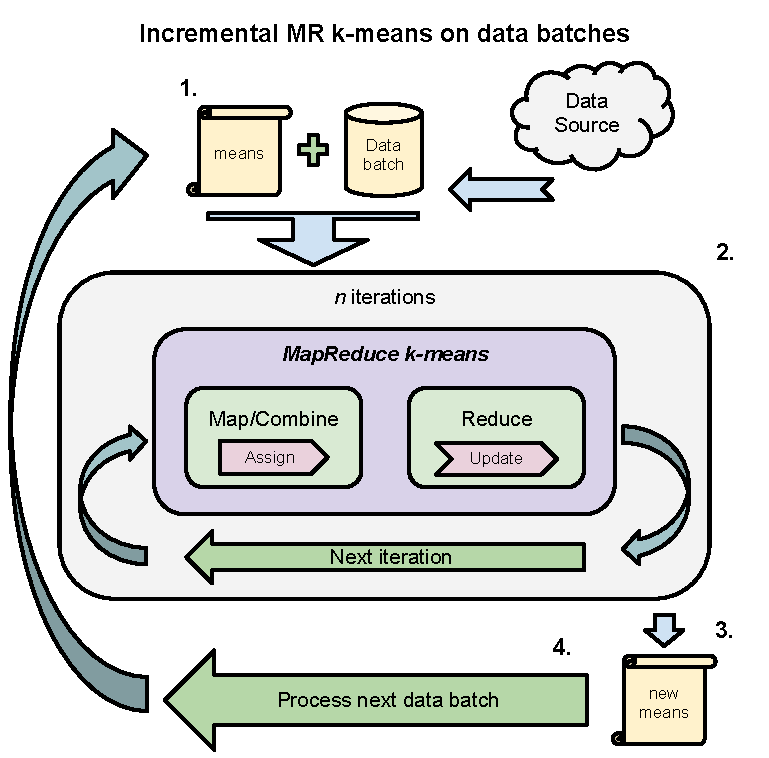
\includegraphics[width=1.0\textwidth]{Figures/IncrementalMRKmeansExecutionProcess.pdf}
\caption{The incremental MR k-means execution flow.}
\label{fig:mrkmeansprocess}
\end{figure}


\section{Development Environment and Tools}
The MapReduce k-means algorithm was implemented using a MR development framework called \textit{mrjob}~\footnote{http://pythonhosted.org/mrjob/}. Mrjob is a open-source Python framework actively maintained by Yelp~\footnote{http://opensource.yelp.com/}, that allows MapReduce jobs to be written in Python 2.5+ and executed on several platforms. Using mrjob allows for rapid implementation of MapReduce jobs by running them locally for development purposes and easily run them on your own Hadoop cluster or even easier using the Amazon Elastic MapReduce (Amazon EMR)\footnote{http://aws.amazon.com/elasticmapreduce/}. Amazon EMR is a web service that allows developers to buy time on a Hadoop cluster to process large-scale data easily and cost-effectively. For the experiments in this thesis we ran our MR k-means algorithm on Amazon EMR web service for scalability tests.

The Python programming language was chosen for this study because GameAnalytics (GA) also uses Python and mrjob to implement their MapReduce jobs. Allowing GA easily to use and build further on the implementation from this study. In this thesis we used the NumPy/SciPy Python library that enables vectorisation approaches and array/matrix data structures for easier and more efficient data vector manipulations. The implementation of algorithms and running experiments were executed on a Linux operating system, recommended by GA instead of using a Windows OS, because of Python libraries compatibility and mrjob.
